\documentclass[a4paper,12pt]{article}
\usepackage[hidelinks]{hyperref}
\usepackage{graphicx}
\usepackage{float}
\usepackage{caption}
\begin{document}
\begin{center}

%Cover page
\Huge\textbf{Functional Requirements(uWatch digital forensic tool)\\}
																											
\vspace{2 cm}

\LARGE\textbf{Group Name:} MPHETamines\newline
 
 
 
 
 
\vspace{0.5 cm}
\begin{tabular}{lr}
Taariq Ghoord&10132806
\\ 
Martha Mohlala&10353403
\\
Phethile Mkhabela&12097561
\\
Sboniso Masilela&%Enter student number
\\
Harrison Maphuti Setati&12310043\\
\end{tabular}

\vspace{1cm}
\textbf{Git repository link:\\}
\url{https://github.com/MPHETamines/MPHETamines/}

\vspace{1cm}
\textbf{Date:} 20 May 2015
\end{center}
\pagenumbering{gobble}
\newpage

%table of contents
\tableofcontents







\newpage
\pagenumbering{arabic}

\section{Introduction}
This document sets out the Software Requirements Specification and Technology Neutral Process Design for the COS 301 group project entitled \textit{Online Neighbourhood Watch(ONW)}.
The aim for this project is to follow a combination of waterfall and agile software development approach within which the application functionality is developed 
iteratively. 
The information provided in this document is presented in such a way as to provide precise and testable requirements. The emphasis is on performing an upfront software 
architecture engineering for iterative stimulation of the detailed requirements for a use case so that each use case can be built, tested and deployed before the detailed 
requirements for the next case are added.
\subsection{Background}
Crime is a prominent issue in South Africa as it is all over the world, Many criminal activities go unresolved or even attended to due to the lack of evidence or concrete witnesses.  Mobile applications have become increasingly popular all over the world and are used in our everyday and work life for common things such as checking the weather; maps for directions and news feed updates.  Digital forensic science hopes to utilise this increasing growth in the use of mobile applications to address the lack of evidence to crime cases in South Africa.
The application is referred to as online neighbourhood watch(ONW) accessible via mobile devices and computers over the internet.  The two main users of the ONW model are the uploader (user of the mobile device) and the forensic investigator or law enforcement agent. 
This tool is to be used by the citizens of South Africa to capture, collect and store potential evidence which can later be viewed and analysed by the Police department and used in the prosecution and detention of criminals.
\subsection{Purpose}
The online neighbourhood watch is aimed to provide a tool that can assist the South African police services(SAPS) reduce crime by enabling the members of the community to be part of the judicial system.  The ONW application captures and stores potential digital evidence of criminal activities which will then be accessed by law enforcement agents and digital forensic investigators.  The goal is to enhance the successful rate of trials and secure a higher number of convictions.
The application can be used in various scenarios, basically it should be used in any setting where a community member feels like a crime has been committed, it is then up to the ONW model to decide if the uploaded data is a potential crime scene. The application should enable a user to capture digital evidence such as digital photographs, audio and video of a potential crime scene in the domain of the ONW to maintain integrity of the data, the data is then stored into the ONW repository.
\subsection{Scope}
The Scope of the ONW is too broad and with the time allocated to the team for this project we decided to focus on only one element of the application, users will only upload pictures as evidence for now and disregard the video and audio part of the ONW model.  There are three aspects of the system the mobile application side, utilised by a community member; the desktop side where a law enforcement agent logs in and the algorithm which sits in between the mobile and desktop.  The algorithm will be used to determine if the photo uploaded is a crime photo. we will focus on human and object detection for now and maybe at a later stage if time permits other media could be uploaded as well. 

\subsection{References}
[List references and controlling documents, including: meeting summaries, white papers, other deliverables, etc.]
\subsection{Assumptions}
[Provide a list of contractual or task level assumptions and/or constraints that are preconditions to preparation of the FRD.  Assumptions are future situations beyond the control of the project, whose outcomes influence the success of a project.]
\subsubsection{Assumptions}
The ONW will be tested around Pretoria Hatfield with the local SAPS precinct. If it passes the test then it will be progressed to other cities in Gauteng, eventually to the whole South Africa. 

\section{Methodology}
[Describe the overall approach used in the determination of the FRD contents.  Describe the modeling method(s) so non-technical readers can understand what they are conveying.]

\section{Functional Requirements}
\subsection{Context}
[Provide a context diagram of the system, with explanations as applicable.  The context of a system refers to the connections and relationships between the system and its environment.]

\subsection{User Requirements}
[Provide requirements of the system, user or business, taking into account all major classes/categories of users.  Provide the type of security or other distinguishing characteristics of each set of users.  List the functional requirements that compose each user requirement.  As the functional requirements are decomposed, the highest level functional requirements are traced to the user requirements.  Inclusion of lower level functional requirements is not mandatory in the traceability to user requirements if the parent requirements are already traced to them.
User requirement information can be in text or process flow format for each major user class that shows what inputs will initiate the system functions, system interactions, and what outputs are expected to be generated by the system.  The scenarios should be comprehensive, to the extent that all user types and all major functions are covered.  Give each user requirement a unique number.  Typically, user requirements have a numbering system that is separate from the functional requirements.  Requirements may be labeled with a leading “U” or other label indicating user requirements.]


\subsection{Use Case Diagrams}

\begin{figure}[H]
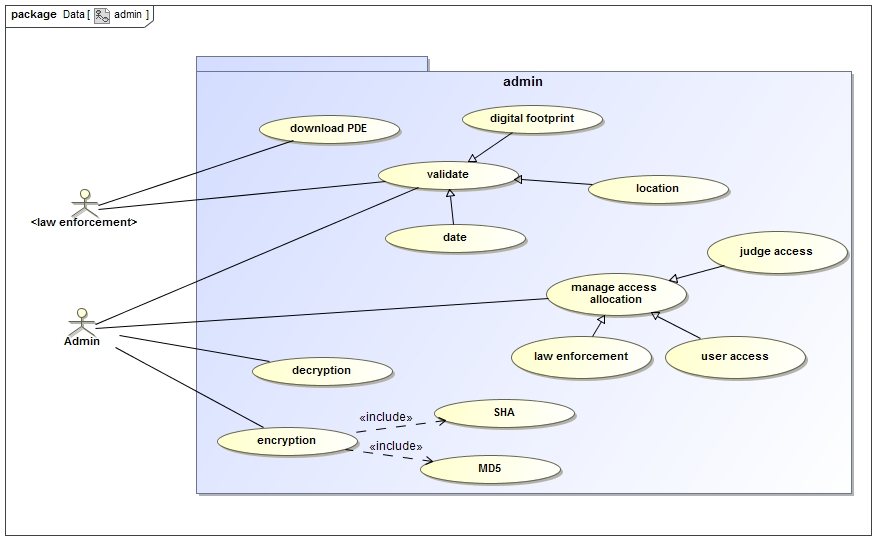
\includegraphics[width=1.0\textwidth]{images/admin.jpg}
\caption{Functional Requirements: Admin/Download Subsystem \label{overflow}}
\end{figure}

\begin{figure}[H]
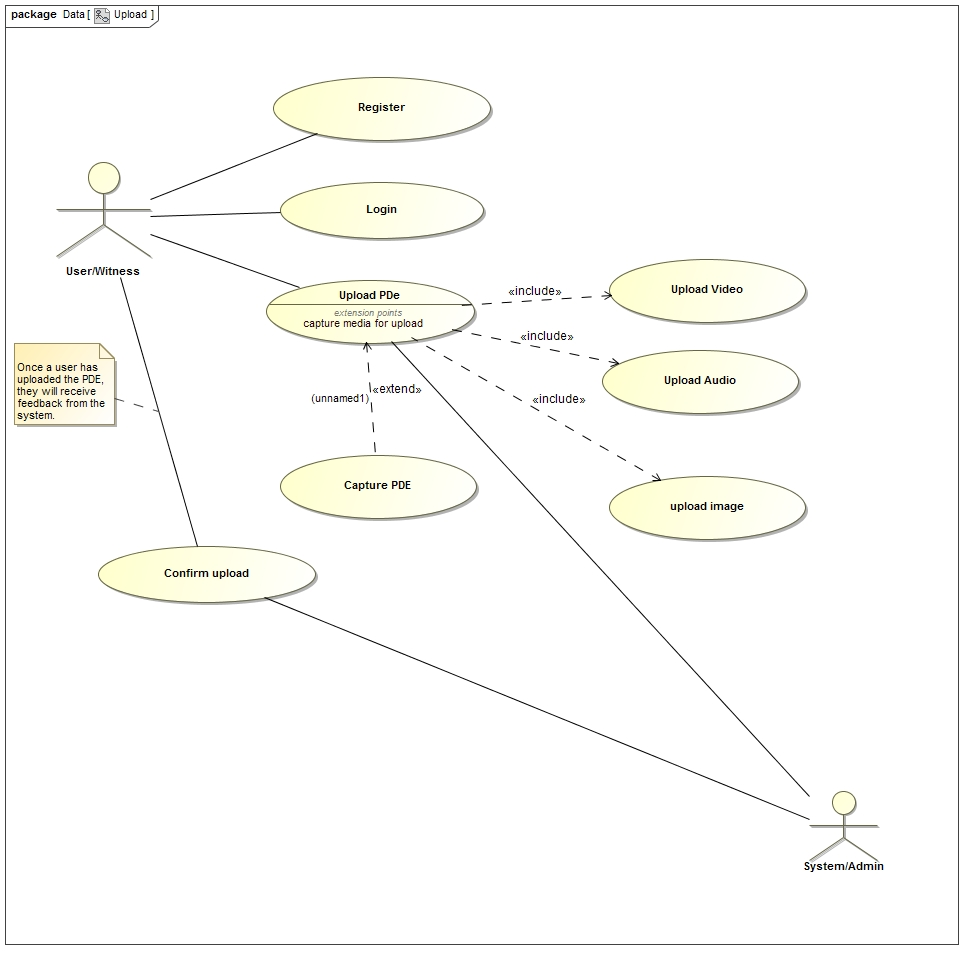
\includegraphics[width=1.0\textwidth]{images/upload.jpg}
\caption{Functional Requirements: Upload Subsystem \label{overflow}}
\end{figure}

\begin{figure}[H]
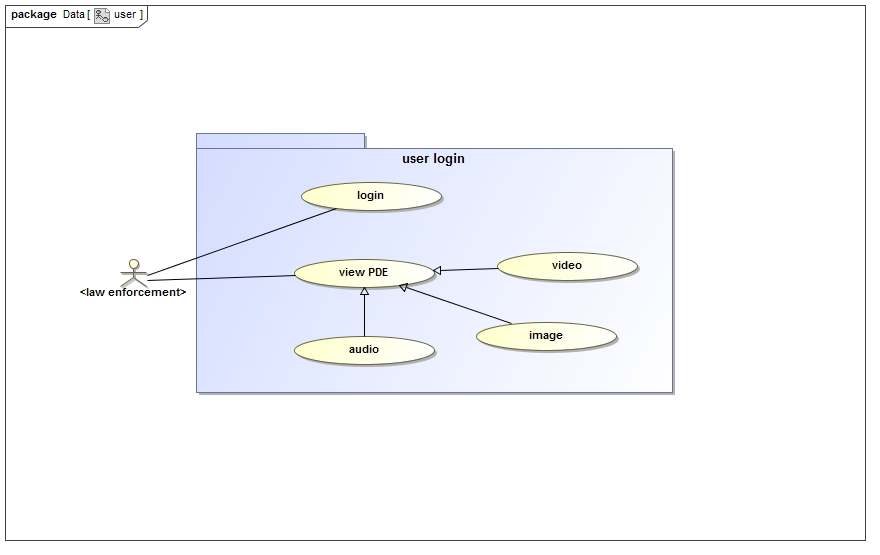
\includegraphics[width=1.0\textwidth]{images/user.jpg}
\caption{Functional Requirements: View Subsystem \label{overflow}}
\end{figure}

\subsection{Class And Sequence Diagrams}
[service contracts and their corresponding sequence diagrams to be shown here]

\subsection{Activity Diagrams}
\begin{figure}[H]
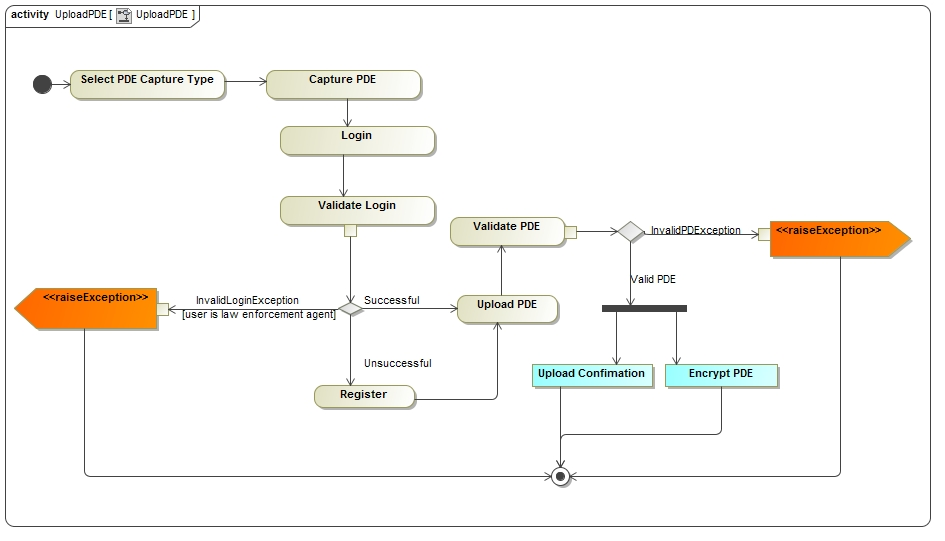
\includegraphics[width=\textwidth]{images/UploadPDE.jpg}
\caption{Process Specification: Uploading Potential Digital Evidence \label{overflow}}
\end{figure}

\begin{figure}[H]
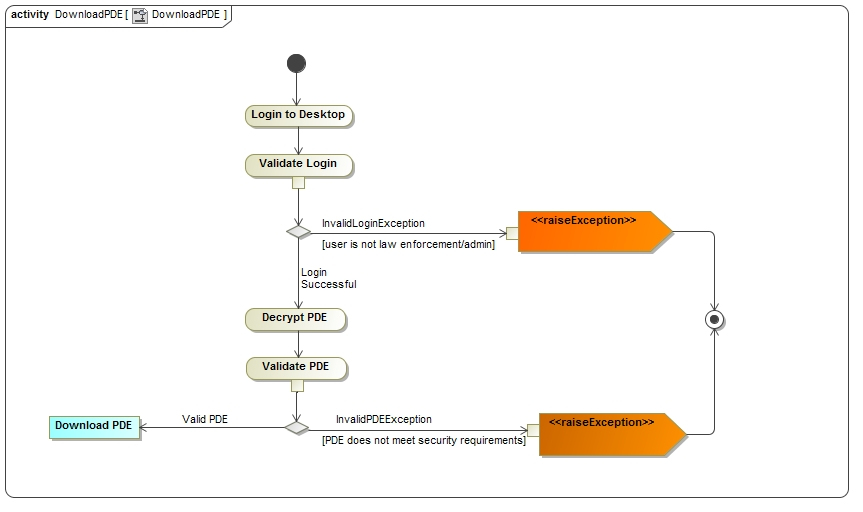
\includegraphics[width=\textwidth]{images/DownloadPDE.jpg}
\caption{Process Specification: Downloading Potential Digital Evidence \label{overflow}}
\end{figure}

\begin{figure}[H]
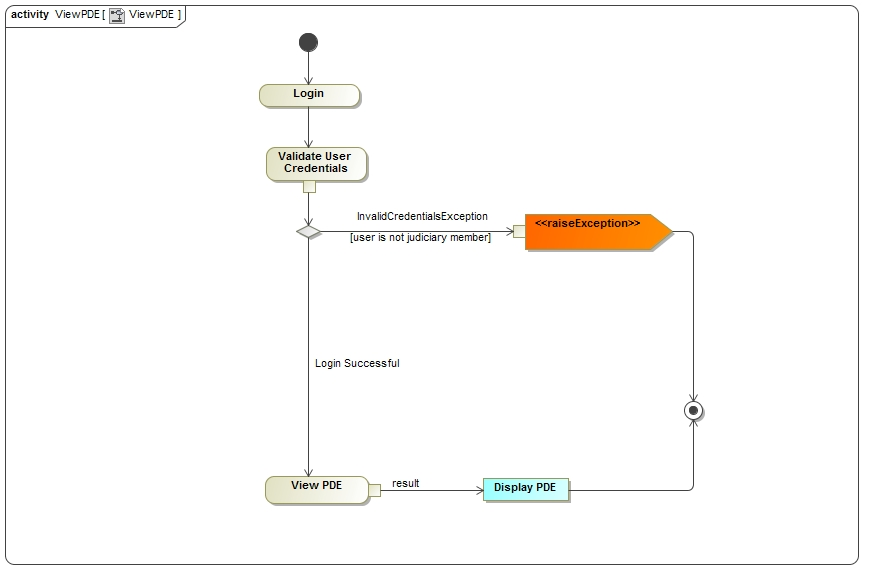
\includegraphics[width=\textwidth]{images/ViewPDE.jpg}
\caption{Process Specification: Viewing Potential Digital Evidence \label{overflow}}
\end{figure}

\subsection{Functional Requirements}
[List the functional requirements of the system.]

\end{document}
